% Name: Grouped bar chart
% Description: Two series side by side for each category, with the values printed on the bars.
% Tags: bar chart, grouped bars, comparison

\usepackage{pgfplots}
\pgfplotsset{compat=1.18}

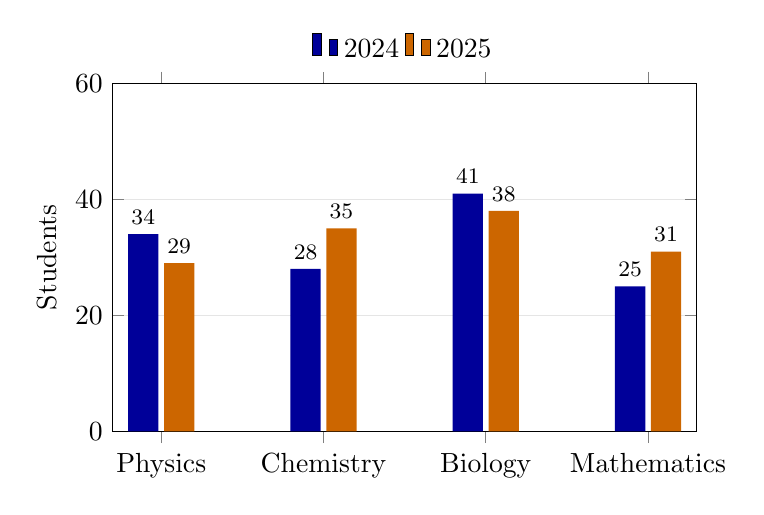
\begin{tikzpicture}
  \begin{axis}[
    ybar, bar width=11pt, ymin=0, ymax=60,
    width=9cm, height=6cm,
    symbolic x coords={Physics, Chemistry, Biology, Mathematics},
    xtick=data, ylabel={Students},
    nodes near coords, nodes near coords style={font=\footnotesize},
    legend style={at={(0.5,1.03)}, anchor=south, legend columns=-1, draw=none},
    ymajorgrids, grid style={gray!20},
  ]
    \addplot[fill=blue!60!black, draw=none] coordinates {(Physics,34) (Chemistry,28) (Biology,41) (Mathematics,25)};
    \addplot[fill=orange!80!black, draw=none] coordinates {(Physics,29) (Chemistry,35) (Biology,38) (Mathematics,31)};
    \legend{2024, 2025}
  \end{axis}
\end{tikzpicture}
